\section{}
% There is a pendulum with mass of 𝑀 connected to a wall with a spring of stiffness 𝑘. Also, there
% is a constant Coulomb friction torque of 𝑇 acting on the pendulum. (Note: Assume that the 𝑓
% oscillations are small).
% a) (5 pts.) Find the time response of the system and maximum angular acceleration of the
% pendulum. (Initial condition: θ = ). π
% 12
% 𝑎𝑛𝑑 θ
% ˙ = 0
% b) (5 pts.) Compare the response of the system with the case where is no friction.
\textit{There is a pendulum with mass of $M$ connected to a wall with a spring of stiffness $k$. Also, there is a constant Coulomb friction torque of $T$ acting on the pendulum. (Note: Assume that the oscillations are small).}
\begin{figure}[H]
    \centering
    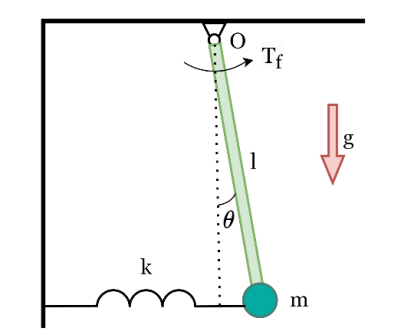
\includegraphics[width=0.5\linewidth]{Questions/Figures/Q5 Problem Diagram.png}
\end{figure}
\begin{enumerate}[label=(\alph*)]
    \item \textit{Find the time response of the system and maximum angular acceleration of the pendulum. (Initial condition: $\theta = \frac{\pi}{12}$ and $\dot{\theta} = 0$)}
    \item \textit{Compare the response of the system with the case where there is no friction.}
\end{enumerate}

\subsection*{Solution}
\subsection{}
The freebody diagram is as follows,
\begin{figure}[H]
    \centering
    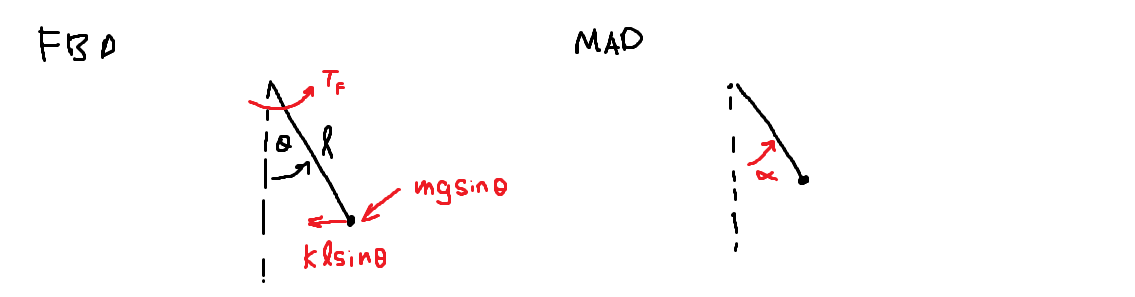
\includegraphics[width=0.8\linewidth]{Questions/Figures/Q5 FBD and MAD.png}
    \caption{Freebody Diagram and Mass Acceleration Diagram}
\end{figure}
The equation of motion is given by,
\begin{align*}
    \circlearrowleft \sum M_{O} &= I_O \ddot{\theta} \\
    &= -k \sin\theta \cos\theta - mgl \sin\theta + T_f 
\end{align*}
Assuming small angle approximation, $\sin\theta \approx \theta$ and $\cos\theta \approx 1$,
\begin{align*}
    \underbrace{ml^2}_{m_{\text{eff}}} \ddot{\theta} + \underbrace{\left(k + mg\right)}_{k_{\text{eff}}} \theta = \underbrace{T_f}_{F_0}
\end{align*}
Assuming $T_f$ is constant, from (7.2),
\begin{align*}
    \theta &= A \sin pt + B \cos pt + \frac{F_0}{k_{\text{eff}}} \\
    \dot{\theta} &= pA \cos pt - pB \sin pt
\end{align*}
Using the initial conditions,
\begin{align*}
    \theta(0) &= \frac{\pi}{12} \\
    \dot{\theta}(0) &= 0 
\end{align*}
First, the initial velocity condition gives,
\begin{align*}
    \dot{\theta}(0) &= pA \cos 0 - pB \sin 0 = 0 \\
    \implies A &= 0
\end{align*}
Now, the initial displacement condition gives,
\begin{align*}
    \theta(0) &= B \cos 0 + \frac{F_0}{k_{\text{eff}}} = \frac{\pi}{12} \\
    \implies B &= \frac{\pi}{12} - \frac{F_0}{k_{\text{eff}}}
\end{align*}
The solution is now,
\begin{empheq}[box=\fbox]{align*}
    \theta(t) &= \left(\frac{\pi}{12} - \frac{F_0}{k_{\text{eff}}}\right) \cos pt + \frac{F_0}{k_{\text{eff}}} 
\end{empheq}
The acceleration is given by,
\begin{align*}
    \ddot{\theta} &= -p^2 \left(\frac{\pi}{12} - \frac{F_0}{k_{\text{eff}}}\right) \cos pt 
\end{align*}
where,
\begin{empheq}[box=\fbox]{align*}
    m_{\text{eff}} &= ml^2 \\
    k_{\text{eff}} &= k + mg \\
    F_0 &= T_f \\
    p &= \sqrt{\frac{k_{\text{eff}}}{m_{\text{eff}}}} 
\end{empheq}
The maximum angular acceleration is given by the amplitude, 
\begin{empheq}[box=\fbox]{align*}
    \big|\ddot{\theta}\big|_{\text{max}} &= \bigg| p^2 \left(\frac{\pi}{12} - \frac{F_0}{k_{\text{eff}}}\right) \bigg|
\end{empheq}

\subsection{}
The response of the system with no friction can be given by letting $T_f =F_0= 0$. The response is then,
\begin{align*}
    \theta(t) &= \left(\frac{\pi}{12} - \frac{0}{k_{\text{eff}}}\right) \cos pt + \frac{0}{k_{\text{eff}}} \\
    &= \boxed{\frac{\pi}{12} \cos pt}
\end{align*}